\section{Sensores}
Para navegar de manera robusta a través de entornos desconocidos y no estructurados, los robots deben poder percibir y modelar su entorno. Es por esto que lo que se busca es construir mapas precisos y ubicarse en los mismos utilizando solo sensores a bordo. Dentro de los mismos pueden diferenciarse dos grandes grupos
\begin{itemize}
    \item En primer lugar, los sensores necesarios para obtener información de los \textit{alrededores} del robot, como pueden ser el LIDAR y la cámara. Estos se los denominan \textit{sensores exteroceptivos}. Un sistema SLAM mínimo requiere al menos de uno de ellos para poder realizar dicha tarea.
    \item Opcionalmente, aquellos sensores que miden el movimiento propio del robot, como pueden ser los acelerómetros y encoders, los que se denominan \textit{sensores propioceptivos}.
\end{itemize}

\subsection{LiDAR}
Light Detection And Ranging, conocido como LiDAR, es una tecnología que tiene su origen en la fusión de la tecnología láser junto con la tecnología RADAR (Radio Detection And Ranging), lo cual ha permitido mejorar en gran medida la precisión de los sistemas de detección, dando lugar a nuevas aplicaciones. Los sensores LIDAR son actualmente una de las opciones más confiables para SLAM robótico tanto en ambientes interiores como exteriores. Los mismos exhibien fuentes y tipos de ruido similares que pueden modelarse libremente como Gaussianos [133].

Muchos investigadores tienen sensores LiDAR de exploración servo-montados en configuraciones de cabeceo [116, 117] o de barrido [118] (Figura \ref{fig:lidars}.a) para producir exploraciones tanto planares como 3D, aunque para este último caso el mismo entrega escaneos cada 1Hz o menos. Este campo de visión, sobre todo el 3D, tiene el costo de una mayor complejidad (sincronización servo temporal) y una menor cobertura en direcciones críticas.
\textbf{[pfingsthron2012] [newman2006] [bosse2009]}

Con el fin de aumentar la frecuencia de recolección de datos, existen sensores que integran múltiples LiDAR en una sola unidad de escaneo (Figura \ref{fig:lidars}.b), de modo que se pueden obtener escaneados en 3D completos a altas velocidades.

\begin{figure}[!b]
    \centering
    \subfloat[Scanse Sweep]{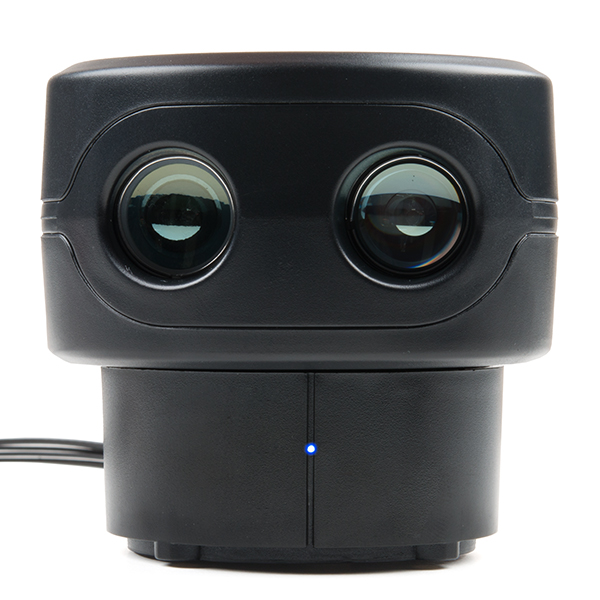
\includegraphics[width=.35\textwidth]{Img/scanse-sweep}}
    \qquad
    \subfloat[Velodyne VLP-16]{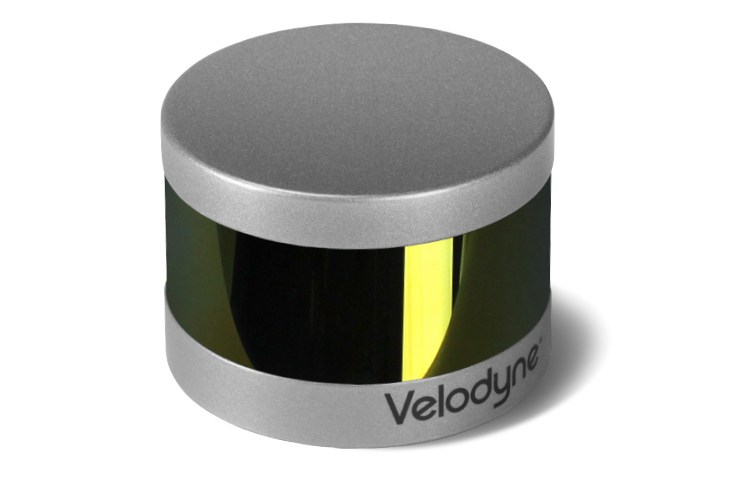
\includegraphics[width=.5\textwidth]{Img/vlp-16}}
    \caption{Algunos LIDAR comerciales}
    \label{fig:lidars}
\end{figure}

\subsubsection{Principio de funcionamiento}
El  fundamento de los dispositivos basados en la tecnología LIDAR es el cálculo del tiempo de vuelo (\textit{ToF - Time  Of Flight}) de los pulsos láser, de manera que, conociendo la velocidad del mismo, las características angulares con las que fue emitido, y la diferencia de tiempos entre el rayo emitido y el reflejado, se puede determinar de manera sencilla la distancia a la que se encuentra el obstáculo/objeto con el que el rayo impactó. Esto permite, con gran exactitud, conocer las coordenadas de la posición de objetos o superficies con respecto del sistema de coordenadas del propio dispositivo.

A medida que cada pulso láser diverge, traza un volumen que es aproximadamente cónico. Si alguna parte de este volumen cónico se cruza con un objeto, parte de la luz reflejada puede regresar a través de la lente del LIDAR. Una vez que la parte frontal del receptor del LIDAR ha recogido suficiente luz (es decir, con un umbral) registra el retorno y calcula la distancia. Esta señal de entrada introduce efectos de acortamiento y alargamiento de rango.

\subsubsection{Fuentes de ruido}
Algunas de las fuentes de ruido que afectan a la medición del LIDAR son
\begin{itemize}
    \item \textit{Ángulo de incidencia:} Si un pulso LIDAR golpea una superficie perpendicularmente, todo el frente de la onda láser se refleja al mismo tiempo. Sin embargo, a medida que aumenta el ángulo de incidencia, parte del frente de onda se refleja antes y la señal recibida activará el umbral, tarde o temprano, dependiendo del diseño del detector frontal. A medida que el ángulo de incidencia se acerca a los 90 grados, una configuración común para el lidar montado horizontalmente, los pulsos lidar viajan casi paralelos al suelo. Estos retornos de ''pastoreo en el suelo'' son extremadamente sensibles al tono del robot, las variaciones en la superficie y otros ruidos. En esta configuración, incluso un robot sin movimiento puede producir mediciones lidar con medidores de ruido de rango. Estos retornos de pastoreo pueden presentar un desafío para SLAM con un lidar montado horizontalmente.
    \item \textit{Efectos de contorno:} están estrechamente relacionados con los retornos de pastoreo, los retornos espurios pueden ocurrir en el límite de los objetos, donde el frente de onda elíptica puede intersecar parte de uno o más objetos a medida que viaja. La medición del rango resultante a menudo se promedia y se crea una medición espuria "colgando" en el espacio vacío entre los objetos. La figura 2.4 demuestra este efecto.
    \item \textit{Propiedades de la superficie del objeto:} causa que la cantidad de luz láser reflejada varíe mucho. Un objeto altamente especular, como un espejo o agua quieta, reflejará la mayor parte de la luz láser y, a menudo, devolverá las mediciones a objetos más distantes (en el rumbo incorrecto). Cuanto más difusamente un objeto refleje la luz, mejor se puede medir en un rango más amplio de ángulos y distancias. Los objetos que absorben la luz infrarroja (que generalmente se ve negra para los humanos) a menudo no pueden reflejar suficiente luz, lo que limita los rangos de medición. Además, en algunos sensores lidar, los objetos blancos pueden aparecer un poco más cerca que los objetos negros, ya que el umbral del receptor se activa un poco antes [133].
    \item \textit{Luz ambiental:} La mayoría de los sensores comerciales LIDAR utilizan filtros de muesca infrarrojos para aumentar la relación señal a ruido. Si bien esto les permite funcionar al aire libre, la luz ambiental intensa, como la luz solar directa, disminuirá su alcance. Cuando la luz reflejada de un pulso lidar no es lo suficientemente fuerte como para activar una medición, un modelo de sensor típico supone que hay espacio libre hasta una fracción del rango máximo del sensor. Esta suposición de espacio libre debe variar según los niveles de luz ambiental, sin embargo, sin sensores adicionales, no es posible determinar cuándo la medición de lidar faltante se debe al espacio libre real o a la luz ambiental excesiva.
    \item \textit{Sincronización temporal:} cuando se monta en un robot en movimiento, el origen de un lidar se moverá a medida que el sensor giratorio complete cada escaneo. Moviéndose a $1m/s$, por ejemplo, un lidar de 40 Hz producirá hasta 25 mm de sesgo si no se compensa. La compensación se puede realizar utilizando un modelo de movimiento continuo, como [134], sin embargo, esto requiere una sincronización rigurosa y una marca de tiempo de los datos del sensor. La figura 2.4 muestra una nube de puntos tridimensional coloreada generada a partir de un lidar montado en un servomotor de movimiento rápido, con una cámara de obturación global y sincronización de microsegundos.
\end{itemize}

\subsubsection{Calibración}
MIRAR

\subsection{Cámara}
Las cámaras en su versión más simple tienen la característica de ser más económicas y sencillas de montar respecto al resto de los sensores utilizados para el SLAM (tal como el LiDAR), además de no emitir señales al entorno para obtener las características del mismo. A la hora de realizar el SLAM. el modelo de sensado de las cámaras consiste básicamente en un mapeo entre el entorno tridimencional y el plano de la imagen bidimensional. Dependiendo del tipo de cámara (monocular, estéreo, omnidireccional, RGB-D, entre otras), es posible utilizar diferentes modelos matemáticos que permitan relacionar puntos del mundo con su respectiva representación en la imagen.

Para las cámaras monoculares, la línea de base entre las imágenes debe estimarse a partir de la odometría, lo que da lugar al problema de SLAM monocular bien estudiado [124, 125]. Otra forma de realizarlo es mediante la percepción de alto nivel, donde se pueden utilizar señales como el tamaño relativo de un objeto para estimar la escala de la imagen y, por lo tanto, la profundidad [126].

En cambio, para las cámaras RGB-D (\textit{D: Depth} - Profundidad) (Figura \ref{fig:camaras}.b), uno de los métodos presentados en la literatura para la realización del SLAM a partir de las mismas [ENDERS2012] consiste en primero extraer características visuales de las imágenes de color entrantes. Luego, se comparan estas características con las características de imágenes anteriores. Al evaluar las imágenes de profundidad en las ubicaciones de estos puntos de características, se obtienen un conjunto de correspondencias 3D puntuales entre dos cuadros cualquiera. Basándose en estas correspondencias, se estima la transformación relativa entre los marcos utilizando RANSAC [TRIVEDI2013].

Por otro lado, las técnicas de visión estéreo utilizan dos cámaras con una separación entre las mismas fija y conocida (Figura \ref{fig:camaras}.a). Las correspondencias de características de la imagen se identifican entre las imágenes mediante la geometría epipolar[REF DE CASTRO] [111], y los rangos se calculan cuando se han medido las disparidades de imagen. Los enfoques pasivos sufren desde muchos modos de falla, desde agujeros de profundidad en áreas de imagen sin características visuales, hasta escenas que crean ambigüedades [123].

\begin{figure}
    \centering
    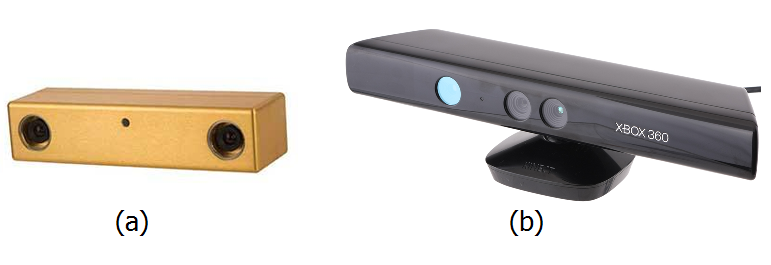
\includegraphics[width=.9\textwidth]{Img/bumblekinect}
    \caption{Cámaras: (a) Bumblebee 2, (b) Kinect}
    \label{fig:camaras}
\end{figure}

\subsection{Sensores Inerciales}
El término sensor inercial se usa para denotar la combinación de un acelerómetro de tres ejes y un giroscopio de tres ejes. Los dispositivos que contienen estos sensores se denominan comúnmente unidades de medición inercial (IMU, por \textit{intertial measurement unit}), los cuales en muchos casos incluyen también un magnetómetro de tres ejes. Estas unidades sensoriales suelen ser usadas para determinar la orientación y posición de objetos a los cuales se encuentran integrados, permitiendo así la incorporación de los mismos en gran número de aplicaciones [7, 59, 109, 156] [DE KOK2017].

Hoy en día, muchos de estos sensores se basan en la tecnología de sistemas microelectromecánicos (MEMS). Los componentes de MEMS son pequeños, ligeros, económicos, tienen un bajo consumo de energía y tiempos de arranque cortos. Su precisión ha aumentado significativamente con los años.

Un giroscopio mide la velocidad angular del sensor, es decir, la velocidad de cambio de la orientación del sensor. En cambio, un acelerómetro mide la fuerza específica externa que actúa sobre el sensor. La fuerza específica consiste tanto en la aceleración del sensor como en la gravedad de la Tierra. Por otro lado, los magnetómetros son los encargados de medir el campo magnético en el que el objeto se encuentra sumergido, obteniendo así información absoluta del ambiente y no referida únicamente al objeto en si. Todos estos sensores tienen el inconveniente de presentar un \textit{bias} variable en el tiempo que afecta su funcionamiento, errores de \textit{scaling} utilizados para convertir las salidas digitales de los sensores en cantidades físicas reales, desalineaciones entre ellos mismos en caso de que se trate de un circuito integrado incluyendo a dos o más de ellos, entre otros.

\subsubsection{Calibración}
En una IMU ideal, los grupos triaxiales deben compartir los mismos ejes de sensibilidad ortogonal 3D que abarcan un espacio tridimensional, mientras que el factor de escala debe convertir la cantidad digital medida por cada sensor en la cantidad física real. Desafortunadamente, las IMU basadas en MEMS de bajo costo generalmente se ven afectadas por el escalado no preciso, las desalineaciones del eje del sensor, las sensibilidades de los ejes cruzados y los sesgos distintos de cero. La calibración de la IMU se refiere al proceso de identificación de estas cantidades.

Sin embargo, las IMUs comerciales de costo elevado presentan también estos problemas (aunque en menor escala), con la diferencia de que el fabricante brinda los datos de la calibración, el cual es único para cada una de ellas, minimizando así los términos de incertidumbre. El factor de calibración de estas IMUs se suele realizar con métodos estándar, comparando los datos arrojados por la IMU con referencias conocidas, haciendo que el proceso sea lento y costoso debido al equipamiento necesario. A continuación se presentarán propuestas para resolver la calibración de los diferentes sensores

\paragraph{Acelerómetro-Giróscopo}
Para evitar el uso de equipamiento específico, en \textbf{[TEDALDI2014]} se propone utilizar solo el movimiento propio de la IMU y sus estados intermedios estáticos para calibrar tanto el giróscopo como el acelerómetro. Este procedimiento explota la idea básica del método de múltiples posiciones, presentado primero en [7] para la calibración de acelerómetros: en una posición estática, las normas de las aceleraciones medidas son iguales a las magnitudes de la gravedad más un multi-factor de error de origen (es decir, incluye \textit{bias}, desalineación, ruido, entre otros). Todas estas cantidades pueden estimarse a través de la minimización sobre un conjunto de actitudes estáticas. 

Después de la calibración de la tríada del acelerómetro, es posible utilizar las posiciones del vector de gravedad medidas por los acelerómetros como referencia para calibrar la tríada del giroscopio. Es por esto que la exactitud de la calibración del giroscopo depende fuertemente de la exactitud de la calibración del acelerómetro. Al integrar las velocidades angulares entre dos posiciones estáticas consecutivas, se consigue estimar las posiciones de gravedad en la nueva orientación. La calibración de los giroscopios finalmente se obtiene minimizando los errores entre estas estimaciones y las referencias de gravedad dadas por los acelerómetros calibrados.

Para una IMU ideal, los 3 ejes de la tríada de acelerómetros y los 3 ejes de la tríada de giroscopios definen un marco tridimensional único, compartido y ortogonal. En la realidad, en base a lo explicado anteriormente, los marcos de los acelerómetros y de los giróscopos no suelen ser ortogonales. A su vez, si se tiene a ambos dentro de un mismo chip, puede definirse un marco del cuerpo (o body frame), el cual es un marco ortogonal que representa, por ejemplo, el chasis del integrado. Este marco suele ser distinto a los otros dos marcos, pero como esta diferencia está dada por ángulos muy pequeños, la medición $\bm{m}$ tanto del acelerómetro como del giróscopo en un marco no ortogonal (o sea, el marco del sensor) puede llevarse al marco del cuerpo mediante
\begin{equation}
    \bm{m}^b = \bm{C}\bm{m}^s
\end{equation}
siendo $\bm{C}$ la matriz de rotación de la Expresión (\ref{eq:rpyinfinitesimal}).

Si se asume que el marco del cuerpo coincide con el marco ortogonal del acelerómetro, entonces para el caso de la aceleración
\begin{equation}
    \bm{a}^b = \bm{C}_a\bm{a}^s
\end{equation}
siendo
\begin{equation}
    \bm{C}_a =
    \begin{bmatrix}
        1 & \alpha_{12} & \alpha_{13} \\
        0 & 1 & \alpha_{23} \\
        0 & 0 & 1
    \end{bmatrix}
\end{equation}
Como se mencionó anteriormente, tanto las mediciones del acelerómetro como las del giróscopo deberían referir al mismo marco de referencia, en este caso, el marco del cuerpo. Por lo tanto,
\begin{equation}
    \bm{\omega}^b = \bm{C}_g\bm{\omega}^s
\end{equation}
siendo
\begin{equation}
    \bm{C}_g =
    \begin{bmatrix}
        1 & \gamma_{12} & \gamma_{13} \\
        \gamma_{21} & 1 & \gamma_{23} \\
        \gamma_{31} & \gamma_{32} & 1
    \end{bmatrix}
\end{equation}

Debido al error de conversión, ambos sensores se encuentran afectados por errores de \textit{scaling}
\begin{align}
    \bm{K}_a &=
    \begin{bmatrix}
        sa_x & 0 & 0 \\
        0 & sa_y & 0 \\
        0 & 0 & sa_z
    \end{bmatrix}
    \\
    \bm{K}_g &=
    \begin{bmatrix}
        sg_x & 0 & 0 \\
        0 & sg_y & 0 \\
        0 & 0 & sg_z
    \end{bmatrix}
\end{align}
 y de \textit{bias}
 \begin{align}
    \bm{b}_a &=
    \begin{bmatrix}
        ba_x \\
        ba_y \\
        ba_z
    \end{bmatrix}
    \\
     \bm{b}_a &=
     \begin{bmatrix}
        bg_x \\
        bg_y \\
        bg_z
     \end{bmatrix}
\end{align}

En consecuente, los modelos completos de los sensores resultan
\begin{align}
    \bm{a}^b &= \bm{C}_a\bm{K}_a\left(\bm{a}^s + \bm{b}_a + \bm{v}_a\right) \\
    \bm{\omega}^b &= \bm{C}_g\bm{K}_g\left(\bm{\omega}^s + \bm{b}_g + \bm{v}_g\right)
\end{align}
con $\bm{v}_i$ correspondiendo a los ruidos de medición de cada uno.

En concreto, para cada uno de los sensores se tendrán parámetros a estimar. Para el caso del acelerómetro
\begin{equation}
    \bm{\epsilon}_{a} = [\alpha_{12},\alpha_{13},\alpha_{23},sa_x,sa_y,sa_z,ba_x,ba_y,ba_z]
\end{equation}

Al aplicarse un promediado a cada intervalo de la calibración del acelerómetro, esto permite olvidar el ruido de la medición, y definir entonces
\begin{equation}
    \bm{a}^b = h(\bm{a}^s,\bm{\epsilon}_{a}) = \bm{T}_a\bm{K}_a(\bm{a}^s+\bm{b}_a)    
\end{equation}

Como en [7], se mueve a la IMU un set de $M$ rotaciones independientes y temporalmente estables, obteniendo entonces $M$ aceleraciones $\bm{a}^s_k$, las cuales son promediadas en cada uno de estos intervalos estáticos. La función de coste para minimizar los parámetros este caso es
\begin{equation}
    \mathscr{S}(\bm{\epsilon}_{a}) = \sum_{k=1}^M(||\bm{g}||^2-||h(\bm{a}^s_k,\bm{\epsilon}_{a})||^2)^2
\end{equation}
donde $||g||^2$ es la magnitud actual del vector de gravedad local, obtenido de tablas específicas. Al tratarse de una regresión no lineal, la misma puede minimizarse utilizando el algoritmo de \textit{Levenberg-Marquardt}.

Para calibrar la triada del giróscopo, puede asumirse al mismo libre de \textit{bias} ya que este sesgo puede obtenerse promediando sobre una cantidad de datos consecutivos de tamaño conveniente en el instante inicial estacionario. Por ello, el vector de parámetro desconocidos resulta
\begin{equation}
    \bm{\epsilon}_{g} = \left[\gamma_{12},\ \gamma_{13},\ \gamma_{21},\ \gamma_{23},\ \gamma_{31},\ \gamma_{32},\ sg_x,\ sg_y,\ sg_z\right]
\end{equation}

Una vez definido el \textit{bias}, como para la calibración del giróscopo se toma al acelerómetro como referencia conocida, se requiere convertir los datos de dicho giróscopo en un vector de aceleraciones. Para ello, se define el operador $\psi$, 
\begin{equation}
    \bm{u}_{g,k} = \psi\left[\bm{\omega}_i^s,\bm{u}_{a,k-1}\right]
\end{equation}
que toma como entrada una secuencia de $n$ lecturas del giróscopo $\bm{\omega}_i^s$ y el versor de gravedad inicial $\bm{u}_{a,k-1}$ obtenido del acelerómetro ya calibrado, y retorna el versor de gravidad final $\bm{u}_{g,k}$. 

Una vez obtenido $\bm{u}_{g,k}$, para el caso del giróscopo, la función de coste será entonces
\begin{equation}
    \mathscr{S}(\bm{\epsilon}_{g}) = \sum_{k=2}^M ||\bm{u}_{a,k} - \bm{u}_{g,k}||^2
\end{equation}
siendo $M$ el número de los intervalos estáticos, $\bm{u}_{a,k}$ es el versor de la aceleración medido promediando en la ventana temporal obtenida en el $k$-ésimo intervalo estático, y $\bm{u}_{g,k}$ corresponde al versor de aceleración en base a los datos del giróscopo computada anteriormente. Se obtiene, entonces, $\bm{\epsilon}_{g}$ minimizando la Expresión anterior utilizando, por ejemplo, el algoritmo de Levenberg-Marquardt.

\subparagraph{Ecuación diferencial ordinaria de la velocidad angular}
Si se tiene un vector $\bm{r}$ de longitud constante, la velocidad angular del mismo en base a las leyes físicas puede obtenerse realizando la derivada del mismo
\begin{equation}
    \frac{d\bm{r}}{dt} = \bm{\omega}\times \bm{r}
\end{equation}
siendo $\times$ el producto externo. Como para el caso evaluado la velocidad angular es perpendicular al vector $\bm{r}$ (producto intero $\bm{\omega}\cdot\bm{r} = 0$), tal como puede verse en la Figura \ref{fig:angularvelocity}. Por lo tanto, puede escribirse a la misma en la forma de cuaterniones
\begin{equation}
    \frac{d\bm{r}}{dt} = \bm{\omega} \otimes \bm{r}
\end{equation}
teniendo en cuenta que tanto $\bm{\omega}$ como $\bm{r}$ se obtienen mediante la Expresión (\ref{eq:vectorquaternionform}).

\textbf{REVISAR SI ESTA BIEN EL GRAFICO, LA IDEA !!!}
\begin{figure}[!ht]
    \centering
    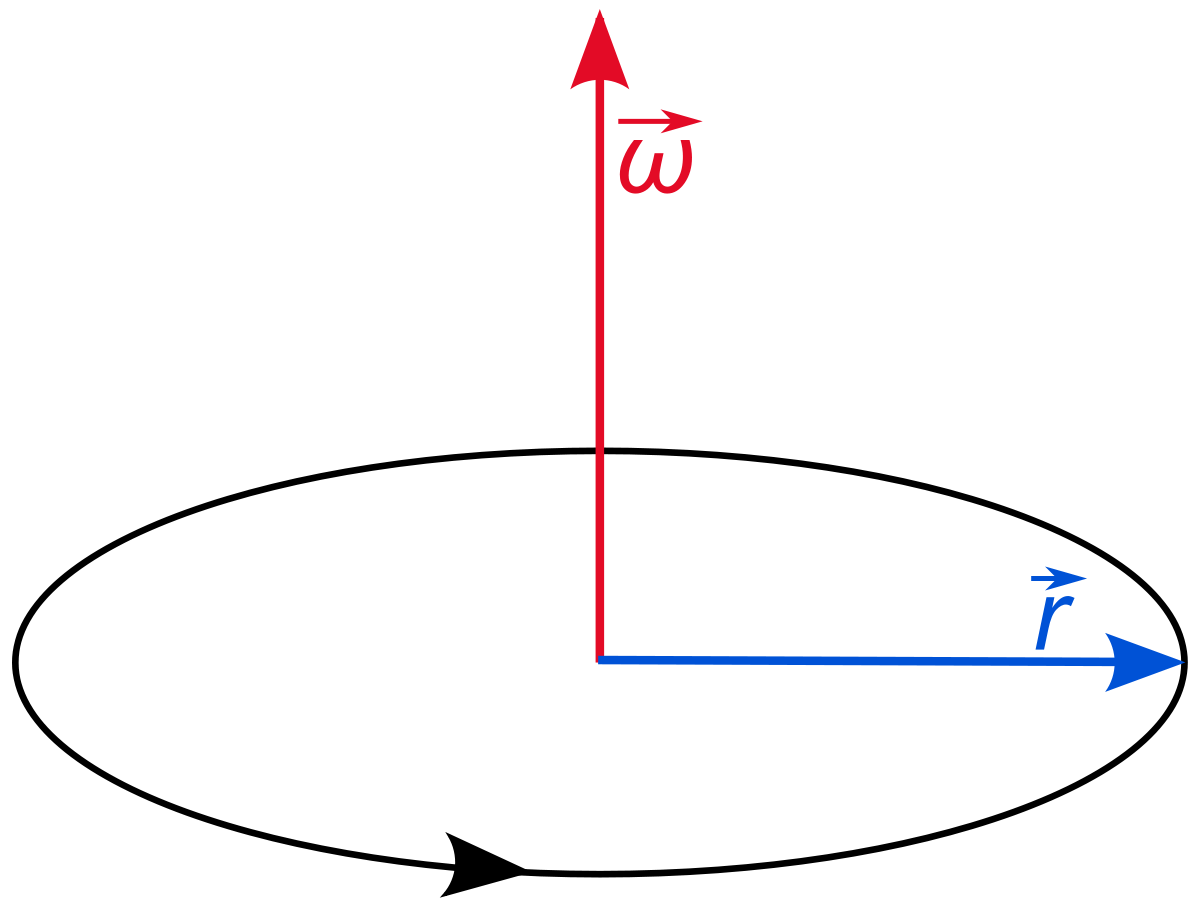
\includegraphics[width=0.5\textwidth]{Img/AngularVelocity.png}
    \caption{Velocidad angular respecto al vector}
    \label{fig:angularvelocity}
\end{figure}

Ahora, siendo que $\bm{r}$ puede definirse mediante la Expresión (\ref{eq:quaternionvectorrotation}), y teniendo en cuenta las propiedades de los cuaterniones
\begin{align}
    \bm{r} &= \bm{q}\otimes \bm{r}_0 \otimes \bm{q}^{-1} \\
    \frac{d\bm{r}}{dt} &= \frac{d}{dt}\left[\bm{q}\otimes\bm{r}_0\otimes\bm{q}^{-1}\right] \\
    &= \dot{\bm{q}}\otimes\bm{r}_0\otimes\bm{q}^{-1} + \bm{q}\otimes\bm{r}_0\otimes\dot{\bm{q}^{-1}} = \bm{\omega}\otimes\bm{r}
\end{align}

Como $\dot{\bm{q}^{-1}}$ puede generar problemas, es posible obtenerlo realizando la derivada del conjugado del cuaternión con su conjugado
\begin{align}
    \frac{d}{dt}\left(\bm{q}\otimes\bm{q}^{-1}\right) &= \frac{d}{dt}1 \\
    \dot{\bm{q}}\otimes\bm{q}^{-1} + \bm{q}\otimes\dot{\bm{q}^{-1}} &= 0
\end{align}
entonces
\begin{equation}
    \dot{\bm{q}^{-1}} = -\bm{q}^{-1}\otimes\dot{\bm{q}}\otimes\bm{q}^{-1}
\end{equation}
sustituyendo y poniéndolo en función de $\bm{r}$
\begin{equation}
        \frac{d}{dt}\left[\bm{q}\otimes\bm{r}_0\otimes\bm{q}^{-1}\right] = \dot{\bm{q}}\otimes\bm{q}^{-1}\otimes\bm{r} - \bm{r}\otimes\dot{\bm{q}}\otimes\bm{q}^{-1}
\end{equation}
donde dicha Expresión tiene la forma de la operación conmutador $\left[\bm{p},\bm{q}\right]$. Finalmente, puede llegarse a la ecuación diferencial
\begin{align}
    \dot{\bm{q}}\otimes\bm{q}^{-1}\otimes\bm{r} - \bm{r}\otimes\dot{\bm{q}}\otimes\bm{q}^{-1} &= \bm{\omega}\otimes\bm{r} \\
    \left[\dot{\bm{q}}\otimes\bm{q}^{-1},\bm{r}\right] &= \bm{\omega}\otimes\bm{r} \\
    2\dot{\bm{q}}\otimes\bm{q}^{-1}\otimes\bm{r} &= \bm{\omega}\otimes\bm{r} \\
    \dot{\bm{q}} &= \frac{1}{2}\bm{\omega}\otimes\bm{q}
\end{align}
donde $\bm{\omega}(t)$ es la velocidad angular en el marco fijo global. En muchos casos es útil expresar la Expresión () en base a la velocidad angular en el marco del sensor. La velocidad angular en este marco es la velocidad angular global rotada en el marco del cuerpo, dado por la Expresión (\ref{eq:quaternionvectorrotation}). En consecuencia,
\begin{equation}
    \dot{\bm{q}} = \frac{1}{2}\bm{q}\otimes\bm{\omega}^s\otimes\bm{q}^{-1}\otimes\bm{q}
\end{equation}
y recordando la Propiedad (\ref{eq:quaternioninverse})
\begin{equation}
    \dot{\bm{q}} = \frac{1}{2}\bm{q}\otimes\bm{\omega}^s 
\end{equation}
Finalmente, en base a la Expresión (\ref{eq:quaternionproductmatrixright}), se llega a
\begin{equation}
    \dot{\bm{q}} = \frac{1}{2}\bm{\Omega}(\bm{\omega}(t))\bm{q}
    \label{eq:edoquaternion}
\end{equation}
siendo $\bm{\Omega}(\bm{\omega}(t))$ la matriz de rotación en base a la velocidad angular obtenida del giróscopo
\begin{equation}
    \bm{\Omega}(\bm{\omega}(t)) =
    \begin{bmatrix}
        0 & -\bm{\omega} \\
        \bm{\omega}^T & -\left[\bm{\omega}\right]_\times
    \end{bmatrix}
    =
    \begin{bmatrix}
        0 & -\omega_x & -\omega_y & -\omega_z \\
        \omega_x & 0 & \omega_z & -\omega_y \\
        \omega_y & -\omega_z & 0 & \omega_x \\
        \omega_z & \omega_y & -\omega_x & 0
    \end{bmatrix}
\end{equation}

\paragraph{Magnetómetro}
Para la calibración del magnetómetro, en cambio, los enfoques tradicionales suponen que hay un sensor de referencia disponible que puede proporcionar información de rumbo precisa. Un ejemplo bien conocido de esto es el balanceo de la brújula [3]. Sin embargo, para permitir que cualquier usuario realice la calibración, se han desarrollado una gran cantidad de enfoques que eliminan la necesidad de una fuente de información de orientación. Una clase de estos algoritmos de calibración de magnetómetro se enfoca en minimizar la diferencia entre la magnitud del campo magnético medido y la del campo magnético local[4]. Este enfoque también se conoce como verificación escalar[5]. Otra clase formula el problema de calibración como un problema de ajuste de elipsoide, es decir, como el problema de mapear un elipsoide de datos a una esfera[6] - [8]. El beneficio de usar esta formulación es que existe una vasta literatura sobre cómo resolver problemas de ajuste de elipsoides,[9][10]. Fuera de estas dos clases, también está disponible un gran número de otros enfoques de calibración[11], donde se consideran diferentes formulaciones del problema de calibración en términos de un problema de máxima verosimilitud. La ventaja de estos métodos es que utilizan sólo la información provista por el magnetómetro.

Sin embargo, si lo que se busca es calibrar un magnetómetro para mejorar la estimación del rumbo en combinación con sensores inerciales, la alineación de los ejes sensoriales de los sensores de inercia y el magnetómetro es crucial en este caso. Se puede ver que esta alineación determina la orientación de la esfera azul de los datos del magnetómetro calibrado en la Fig. 1. Los algoritmos que solo usan datos del magnetómetro pueden asignar el elipsoide rojo de los datos a una esfera, pero sin información adicional, la rotación de esta esfera permanece desconocido.

Varios enfoques más modernos incluyen un segundo paso en el algoritmo de calibración para determinar la desalineación[6], [12] - [14] entre diferentes ejes del sensor. Una opción común para alinear los ejes del sensor de inercia y el magnetómetro es utilizar mediciones de acelerómetro a partir de períodos de aceleraciones bastante pequeñas [12], [13]. La desventaja de este enfoque es que se debe determinar un umbral para usar las mediciones del acelerómetro. Además, se omiten los datos del giroscopio. En [15], por otro lado, el problema se reformula en términos del cambio de orientación, lo que permite el uso directo de los datos del giroscopio. \textbf{[DE KOK 2014]}


\subsection{Encoders}
El objetivo de los encoders es medir las rotaciones relativas de la rueda a la que están asociados. Los encoders normalmente se fijan a la salida del motor o de la caja de cambios, con opciones de diseño que a menudo cambian la resolución angular con la máxima velocidad. Los efectos de resolución y muestreo a menudo producen mediciones ruidosas que requieren filtrado digital. La odometría basada en ruedas supone que no hay deslizamiento entre las ruedas y el terreno. En la práctica, los robots móviles con frecuencia superan la fricción estática y rodante, y cuando una o más ruedas giran o se deslizan, pueden ocurrir grandes errores de odometría. La pendiente del terreno, la fricción y otras propiedades pueden variar, incluso entre ruedas individuales. Los robots de accionamiento diferencial con cuatro ruedas a menudo experimentan grandes errores de odometría cuando giran, ya que se requiere un deslizamiento de las ruedas para girar [150].

\subsection{GPS}
El GPS es un sistema de navegación georreferenciado basado en satélites mediante los cuales estima la latitud, longitud y altitud del objeto en cuestión. Debido a esto, el mismo tiene su campo de aplicación principalmente en ambientes al aire libre, donde mediante la triangulación entre 4 o más satélites puede determinar la ubicación del objeto en cuestión. Debido a esto y a que, entre otros factores, su principio de funcionamiento se basa en medir el tiempo que tardó la señal disparada por un satélite en ser recibida por el propio sensor, el mismo cuenta con precisiones variables dependiendo de la posición de los satélites [162]. Estos sesgos y errores de grandes pasos hacen que la navegación robótica con GPS sea problemática, especialmente con grandes equipos de robots que operan en entornos urbanos y durante muchas horas. [CARLSON2010]